\documentclass[12pt, a4paper, oneside]{article}

%% 包引用
% 定理相关
\usepackage{amsmath, amsthm, amssymb, bm, hyperref, mathrsfs, ctex}

% 页面设置
\usepackage{geometry}
\usepackage{float}
\usepackage{graphicx}
\usepackage{subfigure}%并排子图 共享标题 有子标题
\usepackage[ruled,linesnumbered]{algorithm2e}

% 封面设置
\usepackage{pdfpages}

% 符号说明
\usepackage{longtable}

% 图表绘制
\usepackage[all]{xy}

% tikz绘图相关
\usepackage{tikz}
\usetikzlibrary{math}
\usetikzlibrary{positioning}
\usetikzlibrary{trees}

% 代码
\usepackage{listings}

\def\re{\mathrm{e}}
\def\ri{\mathrm{i}}

\def\Q{\mathbb Q}
\def\M{\mathbb M}
\def\R{\mathbb R}
\def\S{\Bbb S}
\def\N{\Bbb N}
\def\Z{\Bbb Z}
\def\C{\Bbb C}
\def\E{\Bbb E}
\def\P{\Bbb P}
\def\H{\Bbb H}
\def\BS{\Bbb S^2}
\def\Limsup{\varlimsup}
\def\Liminf{\varliminf}

\def\BA{{\bf A}}
\def\BB{{\bf B}}
\def\BC{{\bf C}}
\def\BD{{\bf D}}
\def\BE{{\bf E}}
\def\BF{{\bf F}}
\def\BG{{\bf G}}
\def\BH{{\bf H}}
\def\BI{{\bf I}}
\def\BJ{{\bf J}}
\def\BK{{\bf K}}
\def\BL{{\bf L}}
\def\BM{{\bf M}}
\def\BN{{\bf N}}
\def\BO{{\bf O}}
\def\BP{{\bf P}}
\def\BQ{{\bf Q}}
\def\BR{{\bf R}}
\def\BS{{\bf S}}
\def\BT{{\bf T}}
\def\BU{{\bf U}}
\def\BV{{\bf V}}
\def\BW{{\bf W}}
\def\BX{{\bf X}}
\def\BY{{\bf Y}}
\def\BZ{{\bf Z}}
%
\def\B0{{\bf 0}}  % 定义 \def\B1{{\bf 1}} 有问题
\def\Ba{{\bf a}}
\def\Bb{{\bf b}}
\def\Bc{{\bf c}}
\def\Bd{{\bf d}}
\def\Be{{\bf e}}
\def\Bf{{\bf f}}
\def\Bg{{\bf g}}
\def\Bh{{\bf h}}
\def\Bi{{\bf i}}
\def\Bj{{\bf j}}
\def\Bk{{\bf k}}
\def\Bl{{\bf l}}
\def\Bm{{\bf m}}
\def\Bn{{\bf n}}
\def\Bo{{\bf o}}
\def\Bp{{\bf p}}
\def\Bq{{\bf q}}
\def\Br{{\bf r}}
\def\Bs{{\bf s}}
\def\Bt{{\bf t}}
\def\Bu{{\bf u}}
\def\Bv{{\bf v}}
\def\Bw{{\bf w}}
\def\Bx{{\bf x}}
\def\By{{\bf y}}
\def\Bz{{\bf z}}

\def\BGa{{\bm{\Ga}}}
\def\BGb{{\bm{\Gb}}}
\def\BGg{{\bm{\Gg}}}
\def\BGl{{\bm{\Gl}}}
\def\BGd{{\bm{\Gd}}}
\def\Bxi{{\bm{\xi}}}
\def\Beta{{\bm{\eta}}}
\def\Bnu{{\bm{\nu}}}
\def\Bmu{{\bm{\mu}}}
\def\Beta{{\bm{\eta}}}
\def\Btau{{\bm{\tau}}}
\def\BGvp{{\bm{\Gvp}}}
\def\BGs{{\bm{\Gs}}}
\def\BGt{{\bm{\Gt}}}
\def\Bpsi{{\bm{\psi}}}
\def\Bell{{\bm{\ell}}}

\def\BGP{{\mathbf{\GP}}}
\def\BPsi{{\mathbf{\Psi}}}
%
%

\def\bBA{{\ol{\bf A}}}
\def\bBB{{\ol{\bf B}}}
\def\bBC{{\ol{\bf C}}}
\def\bBD{{\ol{\bf D}}}
\def\bBE{{\ol{\bf E}}}
\def\bBF{{\ol{\bf F}}}
\def\bBG{{\ol{\bf G}}}
\def\bBH{{\ol{\bf H}}}
\def\bBI{{\ol{\bf I}}}
\def\bBJ{{\ol{\bf J}}}
\def\bBK{{\ol{\bf K}}}
\def\bBL{{\ol{\bf L}}}
\def\bBM{{\ol{\bf M}}}
\def\bBN{{\ol{\bf N}}}
\def\bBO{{\ol{\bf O}}}
\def\bBP{{\ol{\bf P}}}
\def\bBQ{{\ol{\bf Q}}}
\def\bBR{{\ol{\bf R}}}
\def\bBS{{\ol{\bf S}}}
\def\bBT{{\ol{\bf T}}}
\def\bBU{{\ol{\bf U}}}
\def\bBV{{\ol{\bf V}}}
\def\bBW{{\ol{\bf W}}}
\def\bBX{{\ol{\bf X}}}
\def\bBY{{\ol{\bf Y}}}
\def\bBZ{{\ol{\bf Z}}}
%
\def\bBa{{\bar{\bf a}}}
\def\bBb{{\bar{\bf b}}}
\def\bBc{{\bar{\bf c}}}
\def\bBd{{\bar{\bf d}}}
\def\bBe{{\bar{\bf e}}}
\def\bBf{{\bar{\bf f}}}
\def\bBg{{\bar{\bf g}}}
\def\bBh{{\bar{\bf h}}}
\def\bBi{{\bar{\bf i}}}
\def\bBj{{\bar{\bf j}}}
\def\bBk{{\bar{\bf k}}}
\def\bBl{{\bar{\bf l}}}
\def\bBm{{\bar{\bf m}}}
\def\bBn{{\bar{\bf n}}}
\def\bBo{{\bar{\bf o}}}
\def\bBp{{\bar{\bf p}}}
\def\bBq{{\bar{\bf q}}}
\def\bBr{{\bar{\bf r}}}
\def\bBs{{\bar{\bf s}}}
\def\bBt{{\bar{\bf t}}}
\def\bBu{{\bar{\bf u}}}
\def\bBv{{\bar{\bf v}}}
\def\bBw{{\bar{\bf w}}}
\def\bBx{{\bar{\bf x}}}
\def\bBy{{\bar{\bf y}}}
\def\bBz{{\bar{\bf z}}}

\def\bBGa{{\bar{\bm{\Ga}}}}
\def\bBGb{{\bar{\bm{\Gb}}}}
\def\bBGg{{\bar{\bm{\Gg}}}}
\def\bBGl{{\bar{\bm{\Gl}}}}
\def\bBGd{{\bar{\bm{\Gd}}}}
\def\bBxi{{\bar{\bm{\xi}}}}
\def\bBeta{{\bar{\bm{\eta}}}}
\def\bBnu{{\bar{\bm{\nu}}}}
\def\bBmu{{\bar{\bm{\mu}}}}
\def\bBeta{{\bar{\bm{\eta}}}}
\def\bBtau{{\bar{\bm{\tau}}}}
\def\bBGvp{{\bar{\bm{\Gvp}}}}
\def\bBpsi{{\bar{\bm{\psi}}}}
\def\bBell{{\bar{\bm{\ell}}}}

\def\bBGP{{\ol{\mathbf{\GP}}}}
\def\bBPsi{{\ol{\mathbf{\Psi}}}}

\def\mb{\mbox}
\def\nnb{\nonumber}
\def\ds{\displaystyle}
\def\cd{\cdot}
\def\cds{\cdots}
\def\all{  \, \forall \, }
\def\ext{ \, \exists \, }
\def\RT{\mathrm{T}}
\def\arccot{{\rm arccot\,}}
\def\wj{{\wedge}}

\def\Llra{\Longleftrightarrow}
\def\Lrla{\Longleftrightarrow}
\def\llra{\longleftrightarrow}
\def\lrla{\longleftrightarrow}
\def\Lla{\Longleftarrow}
\def\Lra{\Longrightarrow}
\def\lra{\longrightarrow}
\def\lla{\longleftarrow}
\def\ra{\rightarrow}
\def\la{\leftarrow}

%%% 自定义命令
%% Tikz符号
% 交换图
\newcommand{\dharrows}[4]{node[Hp={+}] {\tikz\draw[->] (#1)--(#2);}node[Hp={-}] {\tikz\draw[<-] (#1)--(#2);}node[midway,above]{\scriptsize{#3}} node[midway,below]{\scriptsize{#4}}}
\newcommand{\dvarrows}[4]{node[Vp={+}] {\tikz\draw[<-] (#1)--(#2);}node[Vp={-}] {\tikz\draw[->] (#1)--(#2);}node[midway,left ]{\scriptsize{#3}} node[midway,right]{\scriptsize{#4}}}

%% 数学符号
% 微分
\newcommand*{\dif}[1]{\mathrm{d}\mathbf{#1}}

%% 图片相关
\newcommand*{\fig}[3]{
    \begin{figure}[H]
        \centering
        \includegraphics*[scale=#2]{#1}
        \caption{#3}
    \end{figure}
}
\newcommand*{\figsdb}[6]{
\begin{figure}[H]
    \centering
    \setcounter{subfigure}{0}
    \subfigure[#3]{
        \includegraphics[scale=#2]{#1}
    }
    \subfigure[#6]{
        \includegraphics[scale=#5]{#4}
    }
\end{figure}
}
\newcommand*{\figstri}[9]{
\begin{figure}[H]
    \centering
    \setcounter{subfigure}{0}
    \subfigure[#3]{
        \includegraphics[scale=#2]{#1}
    }
    \subfigure[#6]{
        \includegraphics[scale=#5]{#4}
    }
    \subfigure[#9]{
        \includegraphics[scale=#8]{#7}
    }
\end{figure}
}

%% 定理

% 定理样式配置  
\newtheoremstyle{break}  
    {\topsep} % Space above  
    {\topsep} % Space below  
    {\parshape 3 0pt \textwidth 3em \dimexpr\textwidth-3em 1em \dimexpr\textwidth-1em \normalfont} % Body font  
    {} % Indent amount  
    {\normalfont} % Theorem head font  
    {:} % Punctuation after theorem head  
    {\newline} % Space after theorem head  
    {} % Theorem head spec (can be left empty, meaning `normal')  
  
% 定理环境定义  
\newtheorem{remark}{Remark}  
  
\theoremstyle{break}  
\newtheorem{conclusion}{结论}  
\newtheorem{theorem}{定理}  
\newtheorem{example}{例}  
\newtheorem{lemma}{引理}  
\newtheorem*{solving}{解}  

%% Listings配置
% Listings总显示风格
\lstset{
    basicstyle          =   \sffamily,          % 基本代码风格
    keywordstyle        =   \bfseries,          % 关键字风格
    commentstyle        =   \rmfamily\itshape,  % 注释的风格,斜体
    stringstyle         =   \ttfamily,  % 字符串风格
    flexiblecolumns,                % 别问为什么,加上这个
    numbers             =   left,   % 行号的位置在左边
    showspaces          =   false,  % 是否显示空格,显示了有点乱,所以不现实了
    numberstyle         =   \zihao{-5}\ttfamily,    % 行号的样式,小五号,tt等宽字体
    showstringspaces    =   false,
    captionpos          =   t,      % 这段代码的名字所呈现的位置,t指的是top上面
    frame               =   lrtb,   % 显示边框
}

% Listings语言显示风格
\lstdefinestyle{Python}{
    language        =   Python, % 语言选Python
    basicstyle      =   \zihao{-5}\ttfamily,
    numberstyle     =   \zihao{-5}\ttfamily,
    keywordstyle    =   \color{blue},
    keywordstyle    =   [2] \color{teal},
    stringstyle     =   \color{magenta},
    commentstyle    =   \color{red}\ttfamily,
    breaklines      =   true,   % 自动换行,建议不要写太长的行
    columns         =   fixed,  % 如果不加这一句,字间距就不固定,很丑,必须加
    basewidth       =   0.5em,
}


% 文章界面设置

\geometry{a4paper,scale=0.8}
\date{\today}
\linespread{1.5}

\title{Chapter 5 Programming Assignments}
\author{王迦楠\quad 数学科学学院\quad 求数2101\quad 3210105175}
\date{\today}


\begin{document}
\maketitle

restatement of the problem

\paragraph{First Problem}
momentum is “strength or force gained by motion or by a series of 
events.”It directly impacts the player's performance in subsequent points.
To assess the players' performance, it is crucial to have a clear understanding of "momentum." 
We will focus on the following tasks: 
 \begin{enumerate}
    \item determine the influencing factors of "momentum" 
    \item Quantify the variations in "momentum" using fluctuating data.
    \item Visualize the process of "momentum" changes.
\end{enumerate}
 



\section{Model Review}

In this section, we will primarily focus on establishing a model using the Analytic Hierarchy Process (AHP) to address problems 1 and 2. We will break down the problems into five parts:
\begin{enumerate}
\item Problem Analysis
\item Data Cleaning and Processing
\item Collinearity Detection
\item Analytic Hierarchy Process (AHP)
\end{enumerate}

\subsection{Problem Analysis}

% \indent 为了探究"momentum"的原因,我们首先需要对"momentum"有一个初步的定义,"momentum"的大小定义为$$f_{ijk}=\bf{\omega}\cdot\bf{x_{ijk}}$$
% 其中:
% \begin{enumerate}
%     \item $f_{ijk}$代表第i场比赛(按照表格顺序)中第j个point number之前,第k个选手的"momentum"
%     \item $\bf{x_{ijk}}$是一个n维的列向量,代表相对应时刻的一些影响因素,后面我们会具体给出
%     \item $\bf\omega$是一个n维的行向量,指影响因素具体的权重,我们会通过层次分析法来得到
%     \item 这里的公式中,具体会分为两个不同的计算方法,一个分别代表自己发球的场次和对手发球的场次,
%     我们可以写为$$\bf{\omega}=\bf{\omega_0}.\ast {\delta}=(\omega_0^{(0)}
%     \delta^{(0)},\omega_0^{(1)}\delta^{(1)},\dots,\omega_0^{(n)}\delta^{(n)})$$
%     代表两个相同维数向量对应位置相乘构成的向量,其中$\delta$为一个0,1向量,
%     取决于是否是自己的发球轮次,在具体的计算中,我们会分两种情况带入具体考虑。\\
% \end{enumerate}

\indent To investigate the reasons behind "momentum," we first need to provide a preliminary definition for "momentum." The magnitude of "momentum" is defined as $$f_{ijk}=\boldsymbol{\omega}\cdot\boldsymbol{x_{ijk}}$$
where:
\begin{enumerate}
    \item $f_{ijk}$ represents the "momentum" of player $k$ before the $j$th point number in the $i$th match (in the order given by the table).
    \item $\boldsymbol{x_{ijk}}$ is an $n$-dimensional column vector representing some influencing factors at the corresponding moment. Specific details will be provided later.
    \item $\boldsymbol{\omega}$ is an $n$-dimensional row vector indicating the specific weights of the influencing factors, which will be obtained through the Analytic Hierarchy Process (AHP).
    \item In this formula, there are two different calculation methods, one representing rounds where the player serves and the other representing rounds where the opponent serves. We can express it as $$\boldsymbol{\omega}=\boldsymbol{\omega_0} \circ \boldsymbol{\delta}=(\omega_0^{(0)}\delta^{(0)},\omega_0^{(1)}\delta^{(1)},\dots,\omega_0^{(n)}\delta^{(n)})$$ representing a vector formed by element-wise multiplication of two vectors of the same dimension. Here, $\boldsymbol{\delta}$ is a $0,1$ vector indicating whether it is the player's serving round. In the specific calculation, we will consider two cases separately.
\end{enumerate}

% 对于$\bf{x_{ij}^{n}}$的具体定义,我们认为,除了文章中所提到的是否为发球方,还有许多其他因素
% 会造成影响,包括选手的技术,疲惫程度,以及比赛的实时心态等(这里我们主要考虑以上三点)。
% 基于以上三个大点,我们整理了12个因素来作为初步的影响因素,具体如下:

For the specific definition of $\boldsymbol{x_{ij}^{n}}$, we believe that, in addition to whether the player is serving, many other factors can have an impact, including the player's skills, fatigue level, and real-time mental state of the game (here, we mainly consider these three points). Based on these three main aspects, we have organized 12 factors as preliminary influencing factors, as follows:


\subsection{Data Processing and Normalization}

% 在进行数据分析之前,必须保证数据的可用性。如果基于不可靠的数据,
% 无论其价值如何,任何措施都无法提供准确的评估。我们首先去除无用的信息,


\subsection{Collinearity Detection}

% 在对数据进行处理之后,考虑到同一类别的影响因素之间可能存在共线性,比如发球ace,
% 一发得分率,前一分是否得分可能会相关,以及跑动距离,击拍数可能会相关,我们使用stata对数据进行
% 共线性检测。检测结果表面跑动距离与击拍数之间方差膨胀因子较大,因此我们剔除二者之一的击拍数,
% 使用剩下11个数据进行层次分析法。
After processing the data, considering the potential collinearity among factors within the same category, such as serving aces, first-serve scoring rate, and whether the previous point was scored may be correlated, as well as running distance and the number of strokes possibly being related, we conducted collinearity detection using Stata. The results of the detection indicate a significant variance inflation factor between running distance and the number of strokes. Therefore, we decided to exclude one of them, choosing to retain the remaining 11 variables for the Analytic Hierarchy Process (AHP).


\subsection{Analytic Hierarchy Process}
% 我们在之前已经将包含的因素自上而下地分解成若干层次,同一层的诸因素从属于上一层的因素或对上层因素有影响,
% 同时又支配下一层的因素或受到下层因素的作用。从层次结构的第2层开始,我们对影响上一层每个因素,
% 构造比较矩阵,直到最下层。矩阵中的每个元素都显示了相同层次下,因子i和因子j之间的偏好程度。
% 特别要注意的是,我们为两种不同的发球类型(自己发球、对方发球)
% 分别建立了这样的一系列比较矩阵,这里以自己发球为例演示矩阵:

We have previously decomposed the included factors from top to bottom into several levels, where factors within the same level are subordinate to factors in the level above or influence factors in the level above. They also dominate factors in the next level or are influenced by factors in the next level. Starting from the second level of the hierarchy, we construct comparison matrices for each factor influencing the factor in the level above, until reaching the bottom level. Each element in the matrix indicates the preference level between factor i and factor j at the same level. It is essential to note that we have separately established a series of such comparison matrices for two different serving types (serving by oneself and serving by the opponent). Here, we illustrate the matrix using serving by oneself as an example:



\begin{figure}[H]
    \centering
    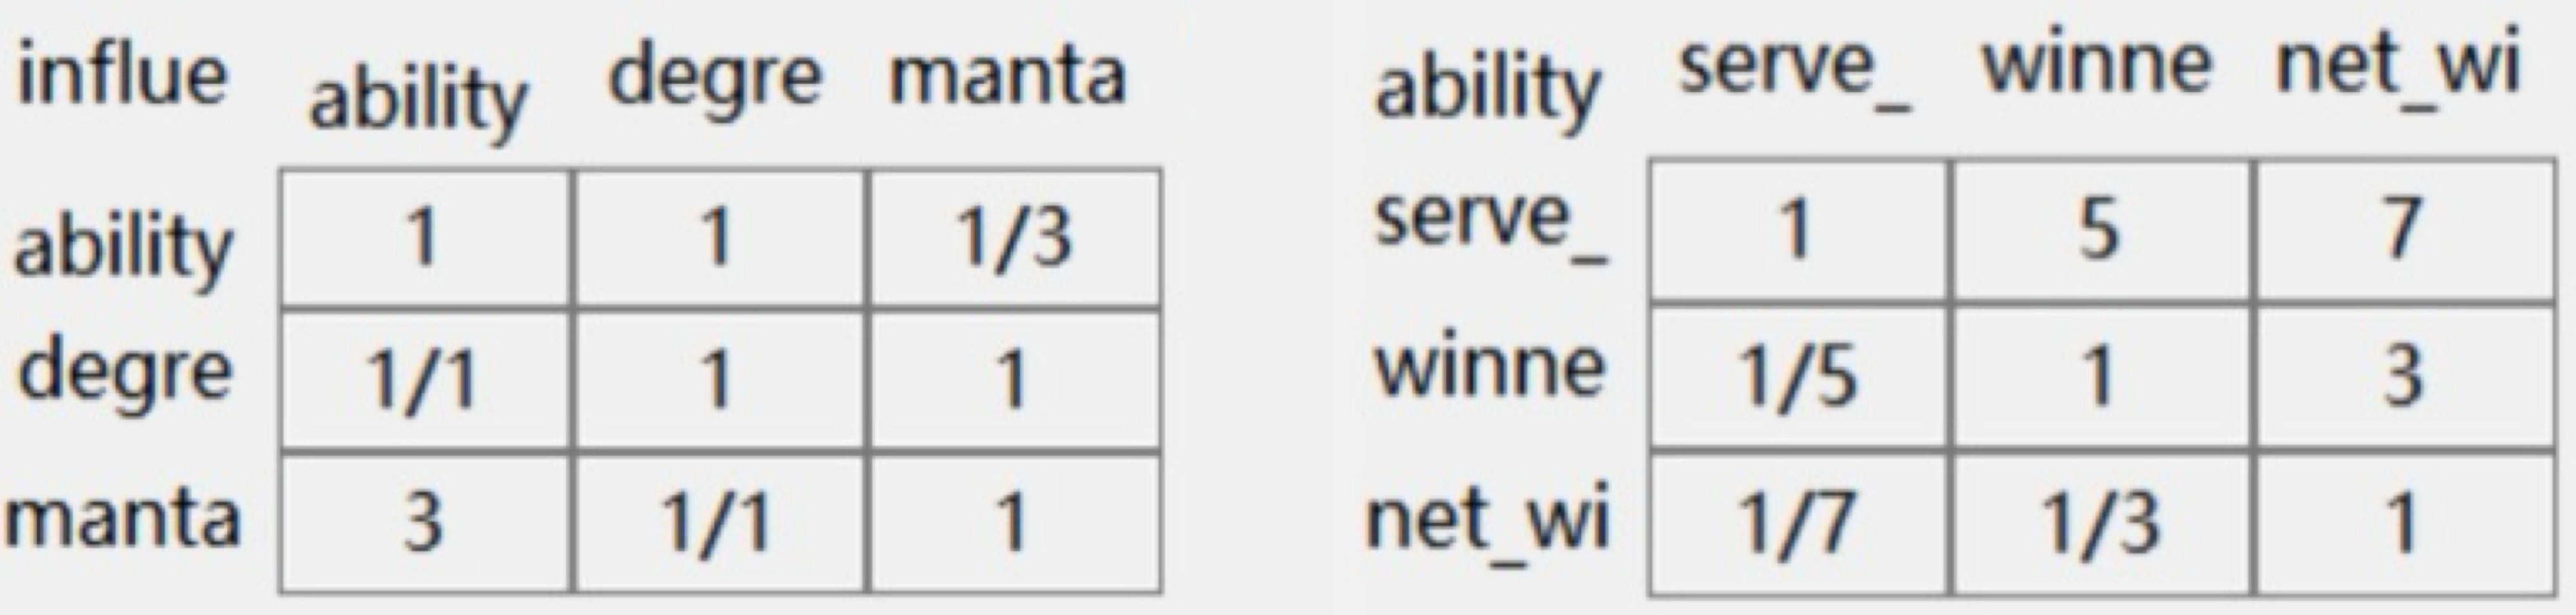
\includegraphics[scale=0.06]{imgs/2.jpg}
    \caption{Comparison matrix for influencing factors and ability}
\end{figure}
\begin{figure}[H]
    \centering
    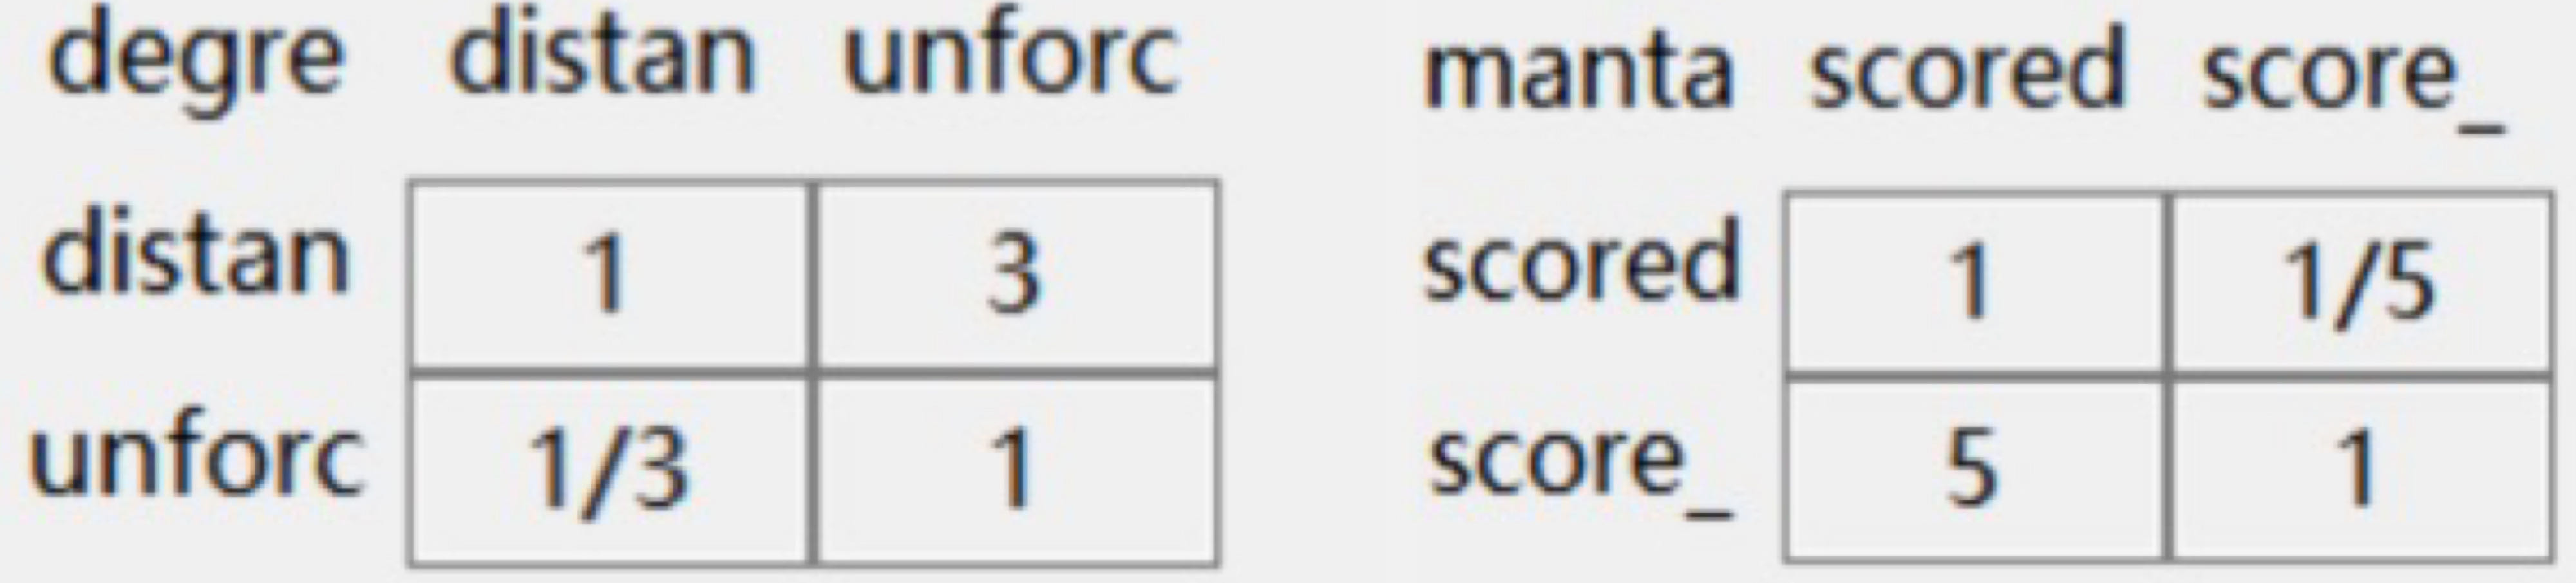
\includegraphics[scale=0.06]{imgs/3.jpg}
    \caption{Comparison matrix for degree of fatigue and mantality}
\end{figure}
\begin{figure}[H]
    \centering
    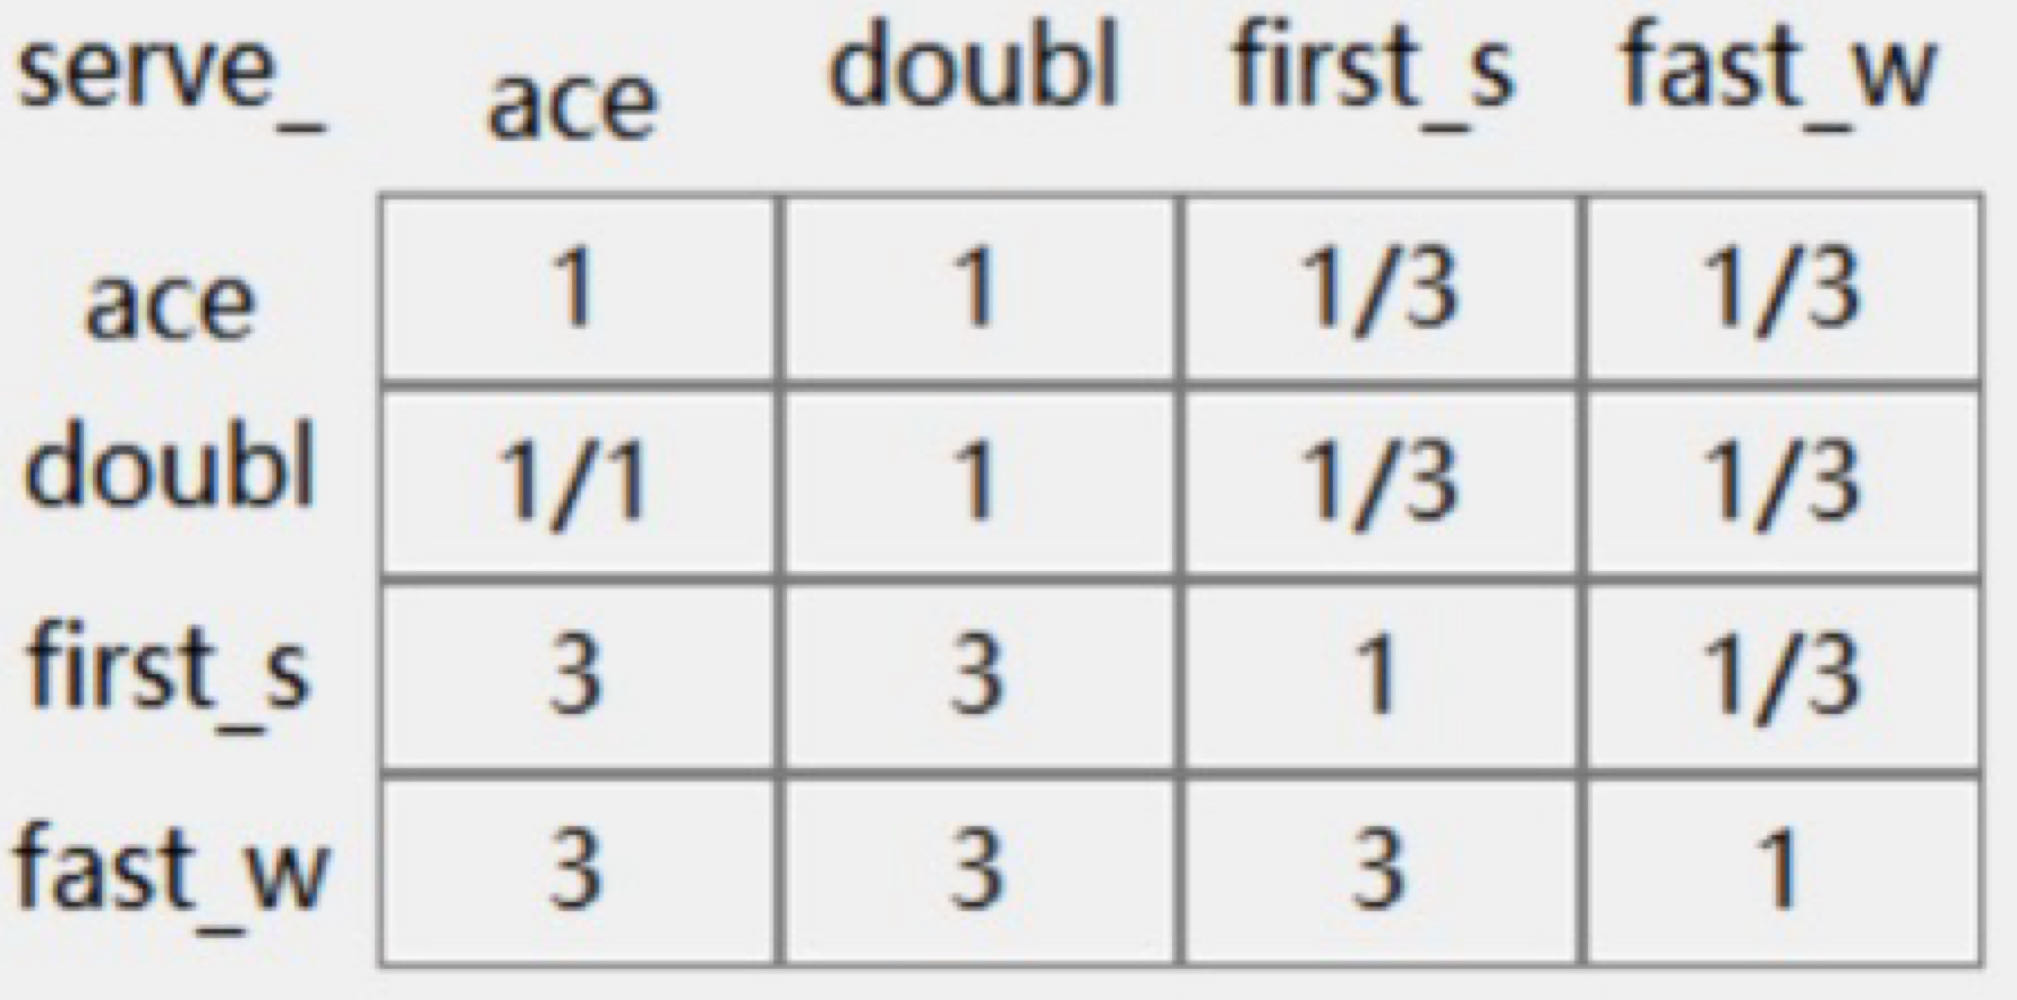
\includegraphics[scale=0.06]{imgs/4.jpg}
    \caption{Comparison matrix for serving}
\end{figure}


% 我们通过计算最大特征值,并对其对应的特征向量进行归一化来获得每个部分的权重。
% 当然,对于每个矩阵,我们首先需要使用组成比(CR)来检验一致性,其中,$CR=\frac{CI}{RI},
% CI=\frac{\lambda_{max}-n}{n-1},RI=0,0.58,0.9(size=2,3,4)$,计算得到的矩阵组成比依次是0.076,0.037,
% 0,0,0.046,因为它们都小于0.1,所以证实了矩阵的一致性。\\

% \indent 因此,我们的模型权重依次为:

We obtain the weights for each component by calculating the maximum eigenvalue and normalizing its corresponding eigenvector. Certainly, for each matrix, we first need to test consistency using the Consistency Ratio (CR), where \(CR=\frac{CI}{RI}\), \(CI=\frac{\lambda_{max}-n}{n-1}\), \(RI=0.0, 0.58, 0.9\) (for matrices of size \(2, 3, 4\)). The computed Consistency Ratios for the matrices are 0.076, 0.037, 0.0, 0.0, 0.046. Since they are all less than 0.1, it confirms the consistency of the matrices.\\

\indent Therefore, the weights for our model are as follows:


\begin{figure}[H]
    \centering
    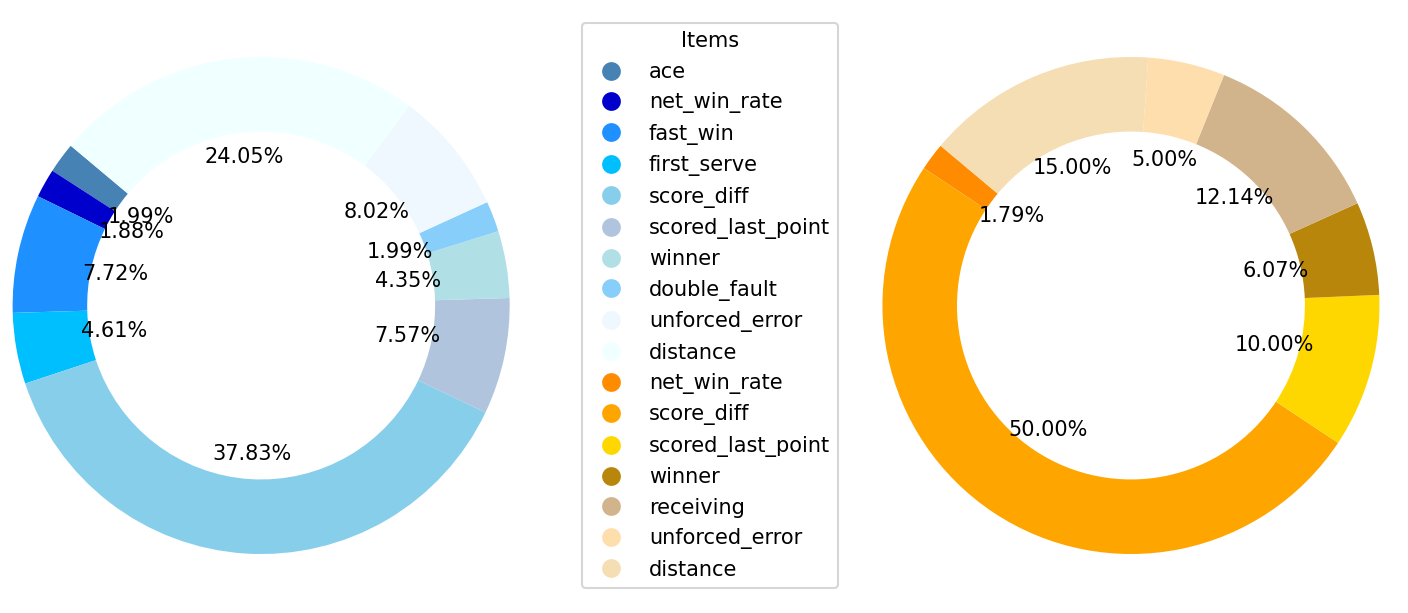
\includegraphics[scale=0.65]{imgs/7.png}
    \caption{Weights in two different situations}
\end{figure}

% 分析图表中各因素发现,影响程度最大的是前一个point是否得分,其次是运动距离,这也非常符合我们的常识。

Analyzing the various factors in the chart, it is evident that the most impactful factor is whether the previous point was scored. Following closely is the distance covered during the play, which aligns well with common intuition.\\


Thus, our final momentum is defined as:(need to change symbol)
$$momentum=\begin{cases}
    \sum\limits_{n=1,n\neq 5}^{11}\omega_n x_n, & \text{if the player serves}  \\
    \sum\limits_{n=5}^{11}\omega_n x_n, & \text{if the opponent serves}
\end{cases}$$
Where $\omega_n(n=1,\dots,11)$ represent the weight of the factors, which is listed in Figure 4.\\

Now, we illustrate the graph of the "momentum" in the first match:


\begin{figure}[H]
    \centering
    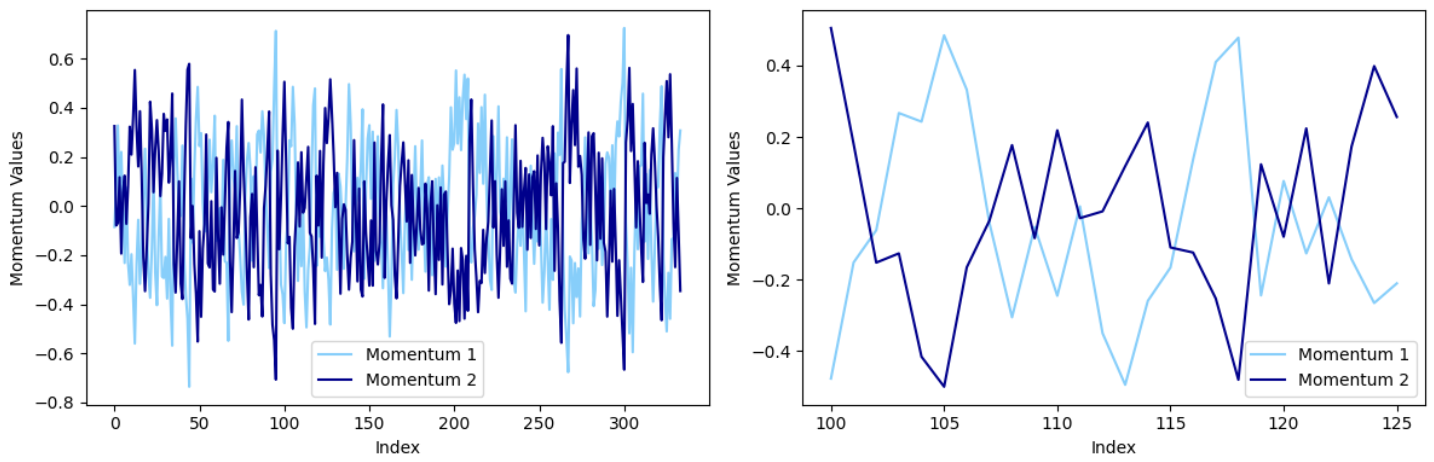
\includegraphics[scale=0.65]{imgs/5.png}
    \caption{Momentum change in the first competition(global and local)}
\end{figure}

% 我们可以发现“momentum”的变化是一个此消彼长的过程。

It can be observed that the variation in "momentum" is a process of give and take.



\end{document}